\subsection{Aprendizado por Reforço Profundo}

O objetivo do Aprendizado por Reforço Profundo (Deep-RL) é controlar um agente na tentativa de maximizar sua função de recompensa.
O algoritmo \textit{Deep Q-Network} \cite{mnih2013playing} foi capaz de desempenhar em nível humano muito dos jogos eletrônicos do Atari por fazer a estimativa das ações de um agente.
Contudo, enquanto a DQN pode resolver problemas em espaços de observações complexos, ela pode apenas lidar com espaços de ações discretos.
E é notável que muitas tarefas, no controle da robótica, têm espaços de ações contínuos.
Então DQN não podem ser aplicadas em domínios contínuos e é necessário usar outros algoritmos capazes de lidar com esse tipo de problema.

\subsubsection{Política de Gradiente Determinística Profunda}

O algoritmo de política de gradiente determinística profunda (DDPG) consiste de um método ator-críticab de política-\textit{off} que usa funções de aproximação que pode aprender políticas de espaço de ação contínuo.
O algoritmo faz uso de uma rede neural para a rede ator e outro para a rede crítica.
Essas duas redes computam a predição de ação para o estado atual e geram um sinal de erro de diferença temporal para cada intervalo de tempo.
A entrada da rede ator é o estado atual, e a saía é um valor real que representa uma ação escolhida para um espaço contínuo de ação.
A saída da crítica é simplesmente o valor de Q estimado do estado atual e ação dada pelo ator.

O maior desafio do aprendizado em espaço de ações contínuas é a exploração. 
Para enfrentar esse desafio é preciso construir a política de exploração $\mu'$ pela adição da amostra de ruído de um processo de ruído $\mathcal{N}$ para a política da rede ator, que é definida como:
\begin{equation}
    \mu' = \mu(s_t) + \mathcal{N}
\end{equation}

Onde $\mathcal{N}$ pode ser escolhido de um jeito que se adéqua ao ambiente. Sendo o processo de Ornstein-Uhlenbeck \cite{uhlenbeck1930theory} o mais usado para gerar eficiência de exploração correlacionada temporalmente em problemas de controle físico.

Em geral, treinar e avaliar a função de política que sai da rede ator e a função de valor que sai da rede crítica, com milhares de trajetórias simuladas correlacionadas temporalmente, leva a introdução de enormes quantidades de variância na aproximação da função verdadeira Q (crítica).
É sugerido usar uma memória de repetição para armazenar as experiências do agente durante o treino \cite{schaul2015prioritized}. 
Isto é, salvar os estados, ações, recompensas e novos estados que o agente explorou durante o episódio.
E então, aleatoriamente selecionar as experiências que vão ser usadas no aprendizado, para assim, quebrar a correlação temporal com os diferentes episódios dos treinos.

A experiência de repetição permite ao agente inteligente aprender de memórias recentes, fazendo com que aumente a velocidade de aprendizado e a quebra de correlações temporais indesejadas. Mesmo com a aplicação de uma memória curta é possível ver uma melhora substancial na desempenho do agente. 
Apesar da aplicação de uma memória de repetição deixar mais lento o aprendizado do agente, se consegue um melhor desempenho dele.

Sem contar a utilização da memória de repetição é preciso fazer uma rede alvo para gerar alvos para que o erro da diferença temporal possa ser regularizado no aprendizado do algoritmo e aumentar a estabilidade. 
A rede alvo é uma rede que possui uma cópia da rede ator e da rede crítica, porém, a sua atualização é feita de um modo “leve”.
Isso quer dizer que a rede alvo não copia diretamente os pesos da rede ator e da rede crítica. 
Os pesos, representado por $\theta$, da rede alvo são atualizados deste modo:
\begin{equation}
    \theta' \leftarrow \tau \theta + (1+\tau)\theta'
\end{equation}

Com $\tau \ll 1$ . Onde o alvo é representado pela apóstrofe.
Então o valores do alvo da rede mudam de forma lenta e assim permitem uma melhora da estabilidade do treinamento.

O algoritmo DDPG é descrito no Algoritmo \ref{alg:ddpg}. Nesta definição é possível ver com mais clareza o algoritmo de aprendizado por reforço profundo. Demonstrando toda etapa de treinamento da rede ator e da rede crítica.

% \begin{algorithm}
% \caption{DDPG com repetição de memória}
% \label{alg:ddpg}
% \begin{algorithmic}
% \STATE Aleatoriamente inicializa a rede crítica $Q(s,a|\theta^Q)$ e a rede ator $\mu(s|\theta^{\mu})$ com os pesos da rede $\theta^Q$ e $\theta^\mu$
% \STATE Inicializa a rede alvo $Q'$  e $\mu'$ com pesos $\theta^{Q'} \leftarrow \theta^Q$, $\theta^{\mu'} \leftarrow \theta^{\mu}$
% \STATE Inicializa a memória de repetição $R$
% \FOR{episódio = 1 até M}
% \STATE Inicializa um processo aleatório $\mathcal{N}$ para a ação de exploração
% \STATE Recebe o estado de observação $s_1$
% \FOR{t = 1 até T}
% \STATE Seleciona a ação $a_t = \mu(s_t|\theta^{\mu})+\mathcal{N}_t$ de acordo com a política atual e ruído de\\ exploração
% \STATE Executa a ação $a_t$ e observa a recompensa $r_t$ e observa o novo estado $s_{t+1}$
% \STATE Armazena a transição $(s_i,a_i,r_i,s_{i+1})$ em $R$
% \STATE Retira um \textit{minibatch} de amostras aleatórias de $N$ transições $(s_t,a_t,r_t,s_{t+1})$ de $R$
% \STATE Define $y_i = r_i + \gamma Q'(s_{i+1}, \mu'(s_{i+1}|\theta^{\mu'})|\theta^{Q'})$
% \ENDFOR
% \ENDFOR
% \end{algorithmic}
% \end{algorithm}

\vspace{1.0cm}
\begin{algorithm}[H]
\DontPrintSemicolon
Aleatoriamente inicializa a rede crítica $Q(s,a|\theta^Q)$ e a rede ator $\mu(s|\theta^{\mu})$ com os pesos da rede $\theta^Q$ e $\theta^\mu$. \;
Inicializa a rede alvo $Q'$  e $\mu'$ com pesos $\theta^{Q'} \leftarrow \theta^Q$, $\theta^{\mu'} \leftarrow \theta^{\mu}$. \;
Inicializa a memória de repetição $\mathcal{R}$.\;
\Para{episódio = 1 até M}{
Inicializa um processo aleatório $\mathcal{N}$ para a ação de exploração. \;
Recebe o estado de observação $s_1$.\;
\Para{t = 1 até T}{
Seleciona a ação $a_t = \mu(s_t|\theta^{\mu})+\mathcal{N}_t$ de acordo com a política atual e ruído de exploração.\;
Executa a ação $a_t$ e observa a recompensa $r_t$ e observa o novo estado $s_{t+1}$.\;
Armazena a transição $(s_t,a_t,r_t,s_{t+1})$ em $\mathcal{R}$.\;
Retira um \textit{minibatch} de amostras aleatórias de $N$ transições $(s_i,a_i,r_i,s_{i+1})$ de $\mathcal{R}$.\;
Define $y_i = r_i + \gamma Q'(s_{i+1}, \mu'(s_{i+1}|\theta^{\mu'})|\theta^{Q'})$. \;
Atualiza a rede crítica minimizando a perda: $L = \frac{1}{N} \sum_{i} (y_i - Q(s_i,a_i | \theta^Q ))^2$.\;
Atualiza a política da rede ator usando o gradiente de política da amostra retirada:\;
\begin{equation*}
    \nabla_{\theta^\mu}J  \approx  \frac{1}{N} \sum_{i} \nabla_a Q( s,a | \theta^Q ) |_{ s=s_i, a=\mu(s_i) } \nabla_{\theta^\mu}\mu( s | \theta^\mu ) |_{s_i}
\end{equation*}
Atualiza a rede alvo:
\begin{gather*}
    \theta^{ Q' } \leftarrow  \tau\theta^Q + ( 1+\tau )\theta^{ Q' }\\
    \theta^{ \mu' } \leftarrow  \tau\theta^\mu + ( 1+\tau )\theta^{ \mu' }
\end{gather*}
}
}
\caption{DDPG com repetição de memória}
\label{alg:ddpg}
\end{algorithm}
\vspace{1.0cm}

% Para melhor que representar o algoritmo, na Figura 4, foi feito um fluxograma de forma a representar o treino da rede DDPG.
% Quando o treino começa as redes crítica, ator e alvo são inicializadas de forma aleatória. 
% O treino dura no total M episódios, onde cada episódio tem T intervalos.

% \begin{figure}[H]
% \caption{Flosefes}
% \centerline{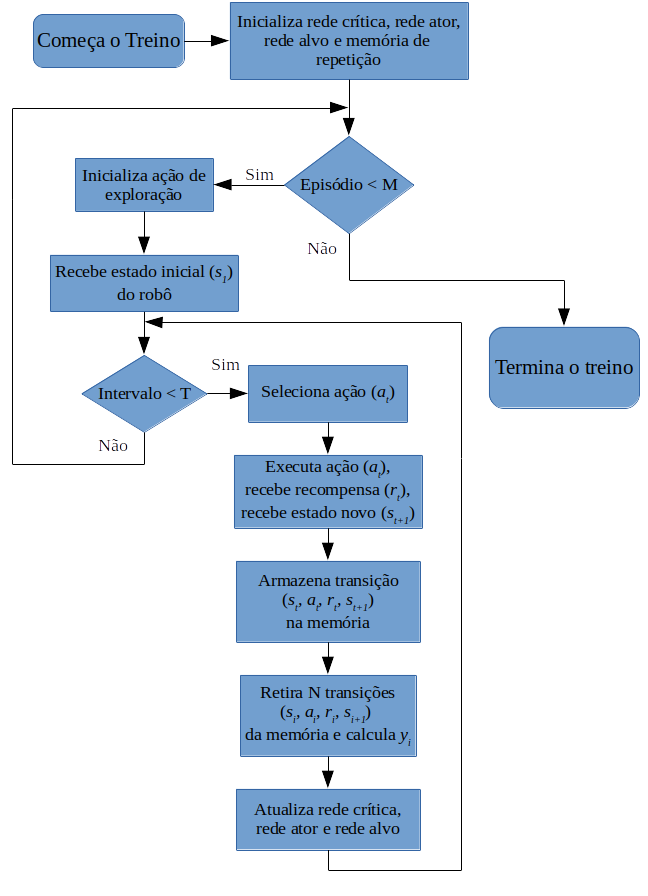
\includegraphics[width=10cm]{imagens/flowchart_ddpg.png}}
% \small{Fonte: Autor}
% \label{fig:flowchart_ddpg}
% \end{figure}

\subsubsection{Ator-Crítica Suave (SAC)}

O Ator-Crítica Suave (SAC) é um algoritmo que otimiza uma política estocástica de um modo de política-\textit{off}. A rede consiste de um método ator-crítica que usa funções de aproximação que podem aprender políticas de ação em espaços contínuos \cite{haarnoja2018soft}.
O algoritmo faz uso de uma rede neural para a rede ator, a rede valor de $V$, e outra para rede crítica.
Essas 3 redes computam a predição de ação para o estado atual e gera um sinal de erro de diferença temporal para cada intervalo de tempo.

A característica central do SAC é a regularização de entropia.
Ao invés de apenas procurar a maximização da recompensa do sistema, a SAC procura também maximizar a entropia da política.
O aumento da entropia resulta é um agente que pode explorar melhor seu ambiente, o que ajuda no aprendizado. E pode prevenir também com que uma política convirja muito cedo para um política local ótima.

A entropia se refere ao quão imprevisível uma variável aleatória pode ser.
Então, se uma variável sempre toma um único valor isso quer dizer que a entropia é considerada zero pois não é nenhum pouco imprevisível.
Uma entropia alta na política explicitamente encoraja a exploração do agente pois é atribuído uma probabilidade igual para a ação que tem o mesmo ou igual valor de $Q$ e assegura que não seja colapsado em repetidamente selecionar uma ação particular do agente.

Para calcular a entropia de $\mathcal{H}$ de uma variável aleatória $x$ de função de densidade $P$, é possível através de:
\begin{equation}
    \mathcal{H}(P) = \mathbb{E}_{x \sim P} [-\log P(x)]
\end{equation}

A rede SAC utiliza dos mesmos métodos de repetição de memória e de uma rede alvo que a rede DDPG. No Algoritmo \ref{alg:sac} é mostrado as etapas de treinamento da rede ator, da rede crítica e da rede de valor $V$ no SAC.

\vspace{1.0cm}
\begin{algorithm}[H]
\DontPrintSemicolon
Aleatoriamente inicializa a rede crítica $Q(s,a|\theta^{Q_{1}})$, $Q(s,a|\theta^{Q_{2}})$, a rede ator $\pi(s,a|\theta^{\pi})$ e a rede de valor de $V(s|\theta^V)$ com os pesos da rede $\theta^{Q_1}$, $\theta^{Q_2}$, $\theta^\pi$ e $\theta^V$. \;

Inicializa a rede alvo $V'$com pesos $\theta^{V'} \leftarrow \theta^V$\;
Inicializa a memória de repetição $\mathcal{R}$.\;

\Para{episódio = 1 até M}{
Recebe o estado de observação $s_1$.\;

\Para{t = 1 até T}{
Seleciona a ação $a_t \sim \pi(s_t,a_t|\theta^{\pi})$ de acordo com a política atual.\;

Executa a ação $a_t$ e observa a recompensa $r_t$ e observa o novo estado $s_{t+1}$.\;

Armazena a transição $(s_t,a_t,r_t,s_{t+1})$ em $\mathcal{R}$.\;

Retira um \textit{minibatch} de amostras aleatórias de $N$ transições $(s_i,a_i,r_i,s_{i+1})$ de $\mathcal{R}$.\;

Computa os alvos para a rede ator $Q$ e  $V$:
\begin{gather*}
    y_q(r_i, s_{i+1}) =  r_i + \gamma V(s_{i+1}|\theta^{V'})
    \\
    y_v (s_i) = \min_{k=1,2} Q(s_i, a_i|\theta^{Q_k}) - \alpha \log \pi (s_i, a_i|\theta^{\pi})
\end{gather*}

Atualiza a rede crítica usando o gradiente
\begin{equation*}
    \nabla_{\theta^Q_k} \frac{1}{|B|} \sum_{(s_i,a_i,r_i,s_{i+1}) \in B} (Q(s_i, a_i|\theta^{Q}_k) - y_q(r_i, s_{i+1}))^2 \qquad \textrm{for}\: k = 1,2 
\end{equation*}

Atualiza a rede valor de $V$ usando o gradiente
\begin{equation*}
    \nabla_{\theta^V} \frac{1}{|B|} \sum_{s_i \in B} (V(s_i|\theta^V) - y_v(s_i))^2
\end{equation*}

Atualiza a política da rede ator usando o gradiente
\begin{equation*}
    \nabla_{\theta^\pi} \frac{1}{|B|} \sum_{s_i \in B} (Q(s_i, a_i|\theta^{\pi}) - \alpha \log \pi (s_i, a_i|\theta^{\pi}))
\end{equation*}

Atualiza a rede valor de $V$ alvo com
\begin{gather*}
    \theta^{ V' } \leftarrow  \tau\theta^V + ( 1+\tau )\theta^{ V' }
\end{gather*}
}
}
\caption{SAC com repetição de memória}
\label{alg:sac}
\end{algorithm}
\vspace{1.0cm}